\documentclass{article}

\usepackage{multicol}
\usepackage{lipsum}
\usepackage{graphicx}
\graphicspath{{images/}}
\usepackage{blindtext}
\usepackage{subfiles} % Best loaded last in the preamble
\usepackage[dvipsnames]{xcolor}
\usepackage[T1]{fontenc}
\usepackage{setspace}
\usepackage{float}

\setlength{\columnsep}{1cm}

\usepackage{fullpage, tikz}
\usepackage{eso-pic}
\AddToShipoutPictureBG{%
	\begin{tikzpicture}[remember picture, overlay]
		\node[opacity=.4, inner sep=0pt]
		at(current page.center){
\includegraphics[width=8.5in, height=11in]{images/background}};
	\end{tikzpicture}%
}

\usepackage[margin={1.5cm,1.5cm}]{geometry}

\newcommand\BackgroundPic{%
	\put(0,0){%
		\parbox[b][\paperheight]{\paperwidth}{%
			\vfill
			\centering
			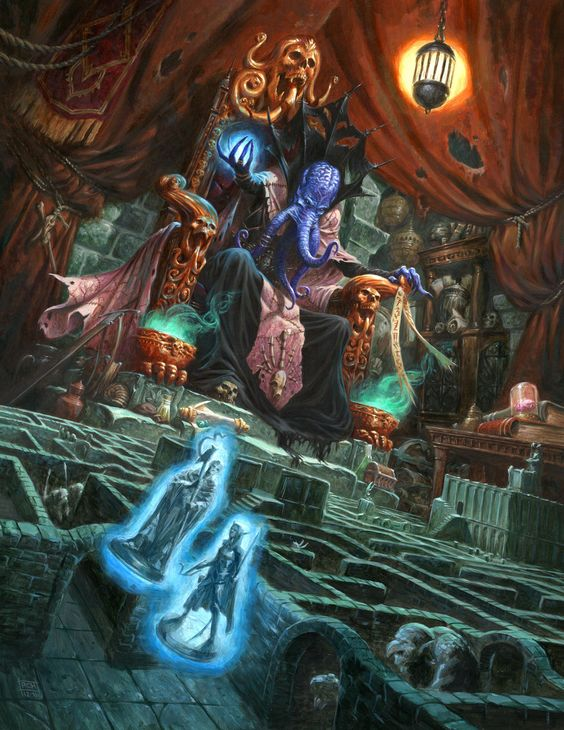
\includegraphics[width=\paperwidth,height=\paperheight]{images/cover.jpg}%
			\vfill
}}}

\title{\color{white}\textsc{\Huge Mystery at Valboro Observatory }}
\date{ }


\setlength\fboxsep{8pt}

\begin{document}
	\AddToShipoutPicture*{\BackgroundPic}
	\maketitle
	\pagebreak
	\begin{multicols*}{2}
	\section{Introduction}
	
		\subsection*{Overview}
		The \emph{Mystery at Valboro Observatory} one-off adventures is meant to be played with a group of NUMPLAYERS players at level PLAYERLEVEL. The adventure is meant to be completed in one session.
		
		The setting for the story is at the Valboro Observatory, on the island of Valboro. A rare astrological event has caused a time rift to open, which is being amplified by the ancient telescope built directly through the mountain. On the other side of the rift, a mysterious figure known as the \emph{Time Harvester} has been using this event to collect and convert time itself as energy.
		
		Time within the observatory itself is at an almost standstill, and once the players find themselves within it, there is no escape from it. The only escape is to breach the rift and defeat the \emph{Time Harvester}.
		
		\subsection*{Background}
		The heroes find themselves on the island of Valboro, known for it's beautiful weather, wealth and vineyards from which is produced the finest quality wine in the know world. The group has been hired by the Winemakers Guild to investigate mysterious circumstances around the famous Valboro Observatory.
		
		The Valboro Observatory is critically important to Valborian society and to the Winemakers Guild because it provides very sophisticated weekly weather reports which contain essential information useful for the local agriculture and wine-making process. The observatory is centuries old and was originally built by brilliant gnomish engineers and scientists, who still operate it to this day. 
		
		The headmaster of the observatory is an older gnome named Frunsmag Karn. The scientists working at the observatory study various meteorological and astronomical sciences to produce finely tuned weekly weather predictions which helps local agriculture and vineyards. The gnomes have owned and operated the observatory for centuries and their trade has been passed down for many generations, making it the most sophisticated weather prediction in the known world.
		
		The observatory is located high up in the Boro mountains, about a three days journey north-west of the coastal capital city of Aleytheas. Built right into the side of a large mountain, it is a marvel of modern engineering and architecture. It is a large cylindrical structure with a domed top containing the main telescope.
		
		\subsection*{Quest}
		For the past month, the Winemakers Guild have grown concerned over the lack of reports or information from the observatory. The Guild sent the Valborian Guard and other mercenaries to investigate but none have returned in weeks. Desperate for this situation to be resolved, the Guild decided to hire off-islander heroes to discover what has transpired at the observatory. The heroes must hurry as every day that passes by without reports is damaging to local farmers and winemakers. The heroes will be handsomely rewarded with a sum of \textbf{10,000 gp} by the Guild for their success.
		
		As the sun sets over the mountains, the adventure begins with the players arriving at the observatory, only to find it eerily abandoned...
		
	\section{The Valboro Observatory}
		Arriving at the observatory, the players stand in front of a long staircase leading to the main entrance to the cylindrical shaped structure. Various broken or abandoned weather measuring devices litter the area around the observatory. The players may choose to investigate the area but there's nothing of value to be found. Since it is built right on the side of the mountain, the terrain around it is extremely treacherous, so there doesn't appear to be any other entrances to the observatory.
		
		The heroes should make their way up the stairs and to the main entrance, which consists of very large and heavy metal doors. The doors are designed to close back up by themselves; once all of the players have passed through the door, they are now trapped in the observatory. 
		
		The air in the observatory smells stale and musty, with a faint smell of death and decay. A quiet humming noise from the generator can be heard, causing the lights to buzz and flicker quickly in the dimly lit rooms.
		
		\subsubsection*{\underline{1. Main Entrance and Foyer}}
	
		
		Trying to leave through the main doors opens up to a mirrored copy of the inside of the observatory. Going in or out of the doors always results in starting back in the main foyer of the observatory.
		
		The foyer consists
		
		
		
	\section{Treasures}

\pagebreak
	
\section{Monsters}

\subsubsection*{Abruhani Pirates}

\subsubsection*{Child of Abruhan Cultist}

\end{multicols*}
	
\end{document}
